% =====================================================================
%  Chapitre 2 -- L'operation de convolution
%  Partie a : definition, calcul pas a pas, vocabulaire, canaux, conventions
% =====================================================================
\section{Chapitre 2 --- L'opération de convolution}

\chapterslide{Chapitre 2}{L'opération de convolution}%
{6 h --- calcul local, noyaux, padding, stride, dimensions}%
{\textbf{Objectifs.} Définir le produit de convolution 2D discret et l'écrire comme un
calcul \emph{local} sur un voisinage ; le mener pas à pas à la main sur une matrice
$5 \times 5$ avec un noyau $3 \times 3$ ; fixer le vocabulaire (noyau, filtre, kernel) ;
traiter une image couleur comme trois canaux ; distinguer enfin convolution et
corrélation croisée, la convention effectivement utilisée par PyTorch.}

\begin{frame}{Plan du chapitre}
\begin{columns}[t]
\begin{column}{0.50\textwidth}
\begin{kbox}[Les cinq temps du chapitre]
\begin{enumerate}
  \item L'opération de convolution : définition et intuition.
  \item Mise en œuvre pas à pas à la main.
  \item Padding, stride, dilatation.
  \item La formule des dimensions et le champ récepteur.
  \item Filtres classiques, 1D, multi-canaux, conventions.
\end{enumerate}
\end{kbox}
\end{column}
\begin{column}{0.46\textwidth}
\begin{ebox}[Ce que vous saurez faire à la fin]
\begin{itemize}
  \item Calculer la sortie d'une convolution $3 \times 3$ à la main.
  \item Prédire la taille de sortie d'une couche convolutive.
  \item Choisir un padding et un stride justifiés.
  \item Écrire et lire une convolution en NumPy / SciPy.
\end{itemize}
\end{ebox}
\end{column}
\end{columns}
\vspace{0.5mm}
\begin{wbox}[La question qui ouvre le chapitre]
Comment fabriquer une opération qui respecte la structure spatiale d'une image,
réutilise les mêmes poids partout, et se calcule vite ? La réponse tient dans une
formule à deux sommes.
\end{wbox}
\end{frame}

\begin{frame}{L'idée : un calcul local sur un voisinage}
\begin{columns}[t]
\begin{column}{0.50\textwidth}
\begin{itemize}
  \item Rappel du chapitre précédent : un neurone dense combine \emph{toutes} les entrées.
  \item Ici, on impose deux contraintes :
  \begin{itemize}
    \item \textbf{localité} : chaque sortie ne regarde qu'une petite fenêtre de l'entrée ;
    \item \textbf{partage de poids} : la \emph{même} fenêtre est réutilisée à chaque position.
  \end{itemize}
  \item La fenêtre est un petit tableau de nombres : le \textbf{noyau}.
  \item On fait glisser ce noyau sur toute l'image ; à chaque position on produit
  \emph{une} valeur de la sortie.
\end{itemize}
\end{column}
\begin{column}{0.46\textwidth}
\begin{abox}[Deux gestes à retenir]
\textbf{1.} Découper une fenêtre de l'entrée.

\textbf{2.} Combiner cette fenêtre et le noyau par une somme pondérée.

\medskip
Le résultat \emph{local} est le point de départ de toute la suite du chapitre :
« convoler » = empiler ce petit calcul répété partout.
\end{abox}
\end{column}
\end{columns}
\end{frame}

\begin{frame}{Définition du produit de convolution 2D}
\begin{columns}[t]
\begin{column}{0.53\textwidth}
Une \textbf{image} $I$ et un \textbf{noyau} $K$ de taille $k_h \times k_w$. Le produit de
convolution discret associe à chaque position $(i,j)$ :
\[
(I \ast K)[i,j] \;=\; \sum_{m=0}^{k_h-1}\ \sum_{n=0}^{k_w-1}
I[i+m,\, j+n]\, K[m,n].
\]
Autrement dit : on \emph{superpose} le noyau au voisinage de $(i,j)$, on fait
\emph{les produits terme à terme}, et on \emph{somme}.
\end{column}
\begin{column}{0.43\textwidth}
\begin{kbox}[Lire la formule]
\begin{itemize}
  \item $I[i+m,\,j+n]$ : une entrée du voisinage.
  \item $K[m,n]$ : le \emph{poids} correspondant du noyau.
  \item Les deux indices parcourent tout le noyau : c'est une double somme de
  $k_h \times k_w$ termes.
\end{itemize}
\end{kbox}
\begin{wbox}[Indices]
L'égalité suppose que $(i,j)$ reste dans l'image et que le voisinage
$(i \dots i+k_h-1,\, j \dots j+k_w-1)$ existe. C'est ce qui impose la taille de sortie
(section suivante).
\end{wbox}
\end{column}
\end{columns}
\end{frame}

\begin{frame}{Vocabulaire : noyau, filtre, kernel}
\begin{columns}[t]
\begin{column}{0.48\textwidth}
\begin{kbox}[Trois noms pour la même chose]
\textbf{NOYAU} (français), \textbf{filtre} (aussi français), \textbf{kernel} (anglais)
désignent le \emph{même} petit tableau de coefficients. Selon les auteurs on lira
aussi \emph{masque} ou \emph{fenêtre}.
\end{kbox}
\begin{abox}[Ce que « filtre » ajoute]
Le mot \emph{filtre} renvoie à l'effet obtenu : lisser, détecter un contour,
accentuer. \emph{Noyau}, lui, désigne uniquement les nombres.
\end{abox}
\end{column}
\begin{column}{0.48\textwidth}
\begin{ebox}[Conventions de nommage en code]
En PyTorch, les poids d'une couche convolutive forment un tenseur d'ordre 4 :
\[
(\text{sortie},\ \text{entrée},\ k_h,\ k_w).
\]
Chaque noyau est donc une petite matrice de coefficients \emph{appris}, un par canal
d'entrée et par canal de sortie.
\end{ebox}
\begin{wbox}[Piège de langage]
« \emph{Le} filtre » d'un CNN n'est pas un filtre classique figé : ses valeurs sont
ajustées par l'apprentissage.
\end{wbox}
\end{column}
\end{columns}
\end{frame}

\begin{frame}{Un exemple complet, en une figure}
\begin{center}
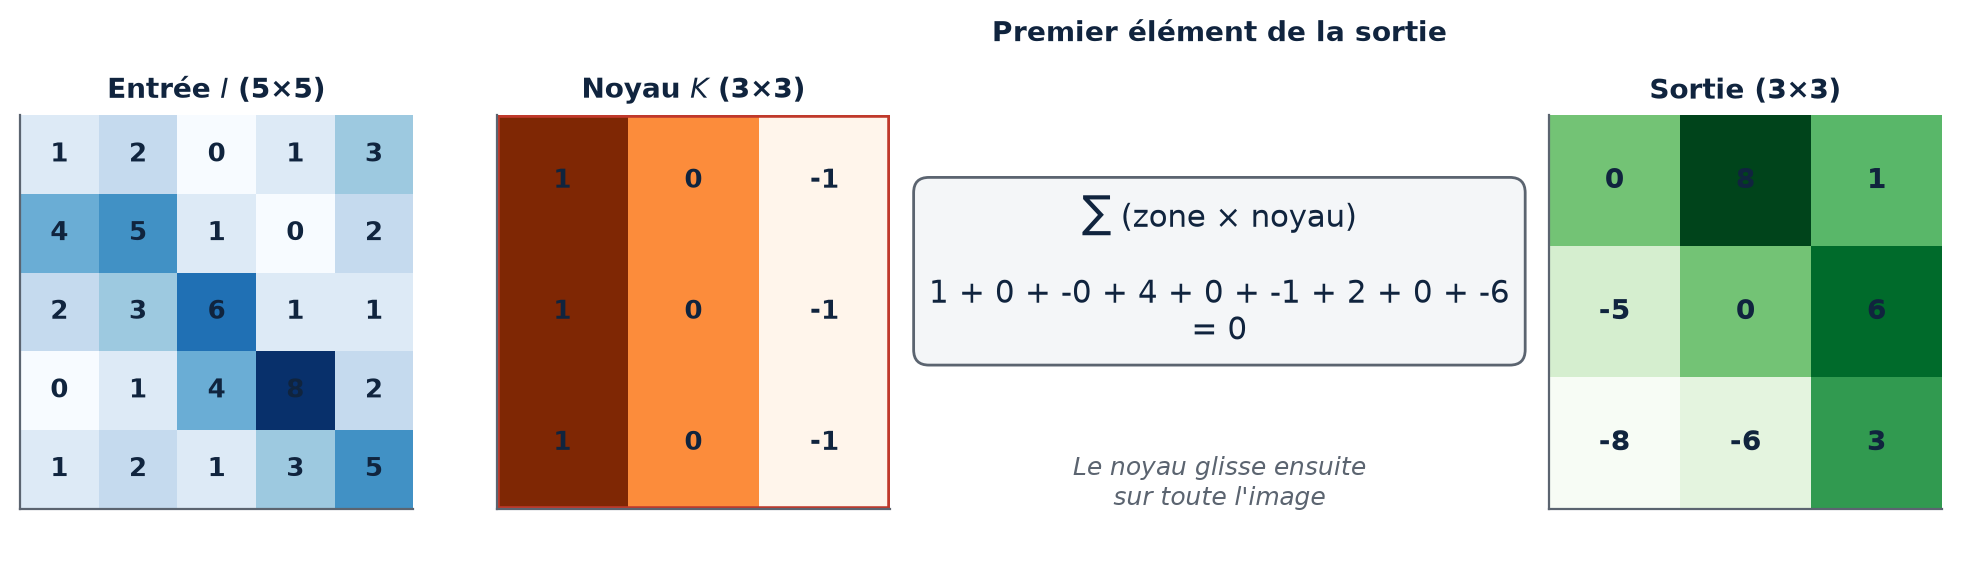
\includegraphics[width=0.93\textwidth]{g01_convolution_pas_a_pas.png}
\end{center}
\vspace{0.5mm}
\begin{kbox}[Ce que montre la figure]
À gauche l'\textbf{entrée} $I$ ($5 \times 5$) ; au centre le \textbf{noyau} $K$
($3 \times 3$) et le calcul du \textbf{premier} élément ; à droite la
\textbf{sortie} ($3 \times 3$). Le premier élément vaut
$1 + 0 + (-0) + 4 + 0 + (-1) + 2 + 0 + (-6) = \mathbf{0}$.
\end{kbox}
\end{frame}

\begin{frame}{Le détail du premier pixel de la sortie}
\begin{columns}[t]
\begin{column}{0.50\textwidth}
Le noyau $\begin{psmallmatrix} 1 & 0 & -1 \\ 1 & 0 & -1 \\ 1 & 0 & -1 \end{psmallmatrix}$
recouvre le coin supérieur gauche de $I$ :
\[
I_{0:3,\,0:3} = \begin{psmallmatrix}
1 & 2 & 0 \\ 4 & 5 & 1 \\ 2 & 3 & 6 \end{psmallmatrix}
\quad\text{et}\quad
K = \begin{psmallmatrix}
1 & 0 & -1 \\ 1 & 0 & -1 \\ 1 & 0 & -1 \end{psmallmatrix}
\]
On multiplie case par case :
\[
1\!\cdot\!1,\ 2\!\cdot\!0,\ 0\!\cdot\!(-1),\ 4\!\cdot\!1,\ 5\!\cdot\!0,\ 1\!\cdot\!(-1),\
2\!\cdot\!1,\ 3\!\cdot\!0,\ 6\!\cdot\!(-1).
\]
\end{column}
\begin{column}{0.46\textwidth}
\begin{solbox}[La somme des neuf produits]
\[
1 + 0 + 0 + 4 + 0 - 1 + 2 + 0 - 6 = 0
\]
\[
(I \ast K)[0,0] = 0
\]
Le \textbf{premier élément de la sortie vaut donc bien $0$}, exactement comme sur la
figure $g01$.
\end{solbox}
\begin{kbox}[Lecture du noyau]
La colonne de $+1$ à gauche et la colonne de $-1$ à droite font une
\emph{différence entre la gauche et la droite} du voisinage : ce noyau détecte une
variation horizontale.
\end{kbox}
\end{column}
\end{columns}
\end{frame}

\begin{frame}{Le noyau balaye toute l'image}
\begin{center}
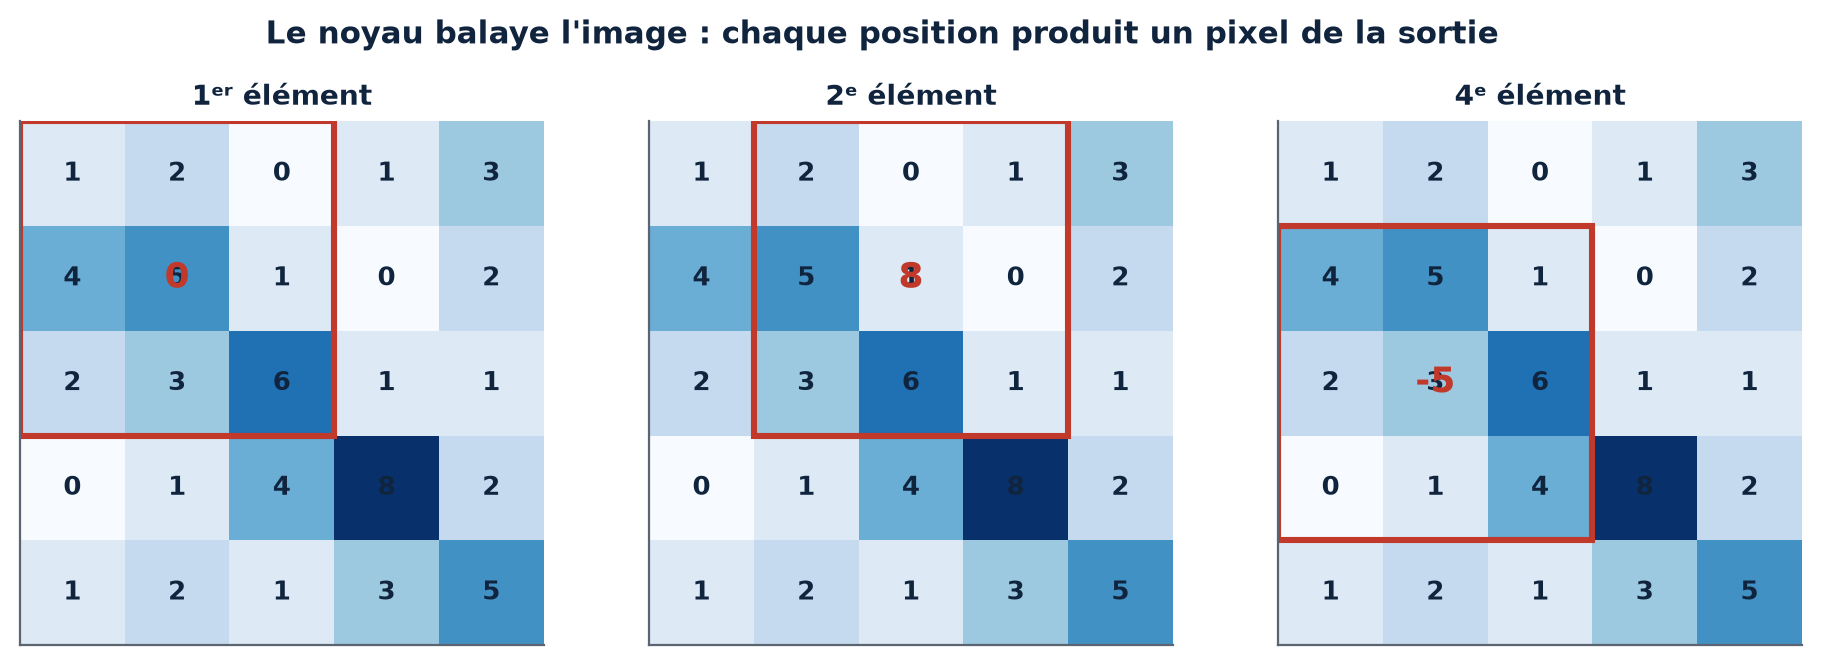
\includegraphics[width=0.90\textwidth]{g02_glissement_noyau.png}
\end{center}
\vspace{0.5mm}
\begin{kbox}[Glissement et sortie]
Posé en haut à gauche, le noyau donne le $1^{\text{er}}$ élément ; décalé d'une colonne,
il donne le $2^{\text{e}}$ ; décalé d'une ligne, le $4^{\text{e}}$. En parcourant toutes
les positions valides d'une image $5 \times 5$, on obtient $3 \times 3 = 9$ valeurs :
\emph{une sortie de même structure spatiale que l'entrée}, mais plus petite.
\end{kbox}
\end{frame}

\begin{frame}[fragile]{Mise en œuvre avec SciPy}
\begin{columns}[t]
\begin{column}{0.55\textwidth}
\begin{codebox}[Deux fonctions, deux conventions]
\begin{lstlisting}
import numpy as np
from scipy.signal import convolve2d, correlate2d

I = np.array([[1, 2, 0, 1, 3],
              [4, 5, 1, 0, 2],
              [2, 3, 6, 1, 1],
              [0, 1, 4, 8, 2],
              [1, 2, 1, 3, 5]])
K = np.array([[ 1, 0, -1],
              [ 1, 0, -1],
              [ 1, 0, -1]])

# convention des CNN (PyTorch) : correlation
s_corr = correlate2d(I, K, mode='valid')
# convolution "vraie" : le noyau est retourne
s_conv = convolve2d(I, K, mode='valid')

print(s_corr.shape)   # (3, 3)
print(s_corr[0, 0])   # 0   -> comme la figure
\end{lstlisting}
\end{codebox}
\end{column}
\begin{column}{0.42\textwidth}
\begin{kbox}[Ce qu'il faut comprendre]
\texttt{mode='valid'} : aucune case n'est ajoutée à l'image, la sortie est donc plus
petite que l'entrée ($5 \times 5 \to 3 \times 3$).
\end{kbox}
\begin{wbox}[Attention]
\texttt{convolve2d} \emph{retourne} le noyau ; \texttt{correlate2d} ne le retourne pas.
Pour un noyau symétrique les deux coïncident ; sinon ils diffèrent (voir plus loin).
\end{wbox}
\end{column}
\end{columns}
\end{frame}

\begin{frame}[fragile]{Vérifier à la main : un noyau sur une matrice $5 \times 5$}
\begin{columns}[t]
\begin{column}{0.55\textwidth}
\begin{codebox}[Recalcul sans bibliothèque, en NumPy]
\begin{lstlisting}
import numpy as np

I = np.array([[1, 2, 0, 1, 3],
              [4, 5, 1, 0, 2],
              [2, 3, 6, 1, 1],
              [0, 1, 4, 8, 2],
              [1, 2, 1, 3, 5]])
K = np.array([[ 1, 0, -1],
              [ 1, 0, -1],
              [ 1, 0, -1]])

sortie = np.zeros((3, 3))
for i in range(3):            # ligne de sortie
    for j in range(3):        # colonne de sortie
        fenetre = I[i:i+3, j:j+3]
        sortie[i, j] = np.sum(fenetre * K)

print(sortie)
print("premier element :", sortie[0, 0])
\end{lstlisting}
\end{codebox}
\end{column}
\begin{column}{0.42\textwidth}
\begin{solbox}[Résultat --- identique à la figure $g01$]
\[
\texttt{sortie} =
\begin{psmallmatrix}
0 & 8 & 1 \\ -5 & 0 & 6 \\ -8 & -6 & 3
\end{psmallmatrix}
\]
\[
\texttt{sortie[0,0]} = 0
\]
Le premier élément vaut bien $\mathbf{0}$. Le reste de la matrice est identique à la
sortie affichée sur la figure.
\end{solbox}
\begin{kbox}[Pourquoi cela marche]
\texttt{I[i:i+3, j:j+3]} découpe exactement le voisinage, \texttt{fenetre * K} fait les
produits terme à terme, \texttt{np.sum} les additionne. C'est la définition appliquée
littéralement.
\end{kbox}
\end{column}
\end{columns}
\end{frame}

\begin{frame}{Trois propriétés utiles}
\begin{columns}[t]
\begin{column}{0.48\textwidth}
\begin{kbox}[Propriétés de la convolution]
\begin{itemize}
  \item \textbf{Linéarité} : $(a I_1 + b I_2) \ast K = a\,(I_1 \ast K) + b\,(I_2 \ast K)$.
  \item \textbf{Commutativité} : $I \ast K = K \ast I$ (l'ordre ne change rien au résultat).
  \item \textbf{Associativité} : $(I \ast K_1) \ast K_2 = I \ast (K_1 \ast K_2)$.
\end{itemize}
\end{kbox}
\end{column}
\begin{column}{0.48\textwidth}
\begin{abox}[Ce que ces propriétés permettent]
\begin{itemize}
  \item Combiner deux petits noyaux en un seul : base de la \emph{convolution
  séparable}.
  \item Réordonner les opérations sans changer le résultat.
  \item Attention : la commutativité \emph{exacte} vaut pour la convolution « vraie »
  (noyau retourné), pas pour la corrélation croisée.
\end{itemize}
\end{abox}
\end{column}
\end{columns}
\vspace{0.5mm}
\begin{wbox}[Réserve importante]
Le CNN n'utilise pas une convolution au sens strict mais une \textbf{corrélation
croisée} : le noyau \emph{n'est pas} retourné. Les propriétés ci-dessus s'énoncent
donc avec les mêmes restrictions de convention.
\end{wbox}
\end{frame}

\begin{frame}{Une image couleur, c'est trois convolutions}
\begin{center}
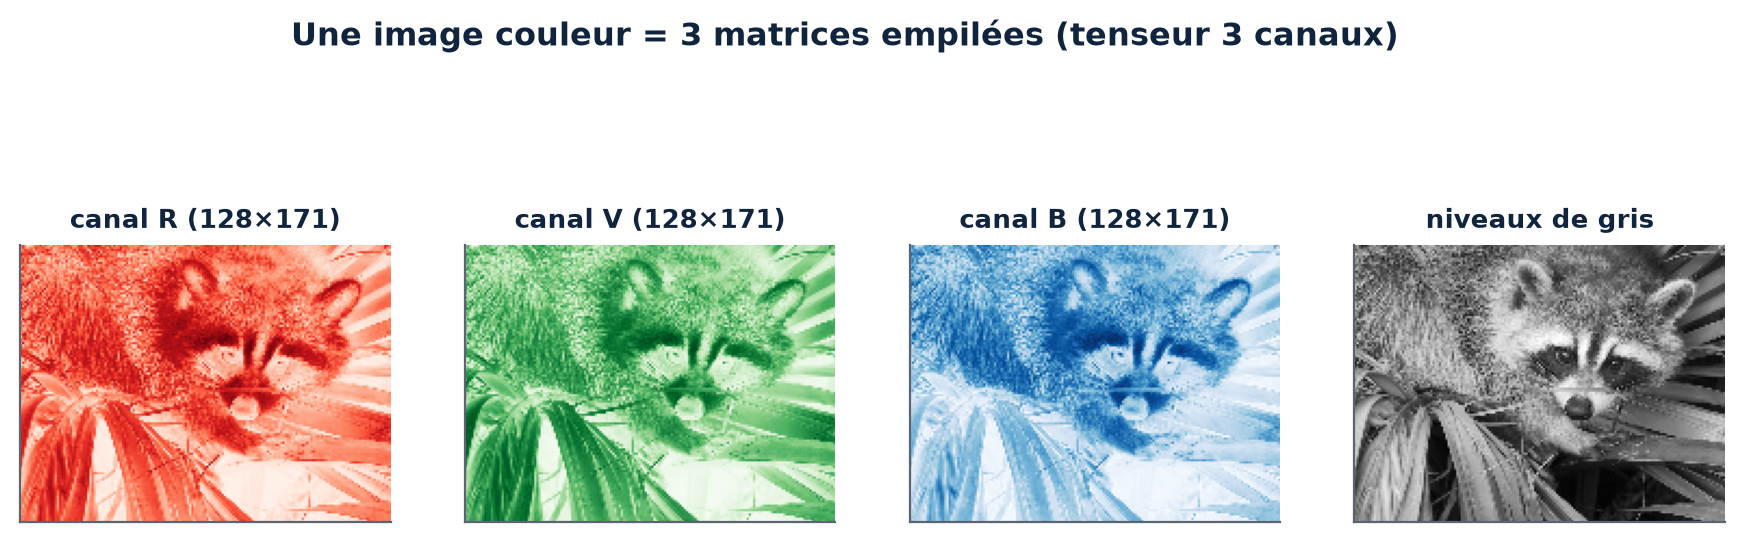
\includegraphics[width=0.92\textwidth]{g10_multicanaux.png}
\end{center}
\vspace{0.5mm}
\begin{kbox}[Du canal à la convolution]
Une image couleur $128 \times 171$ assemblée en RVB est un tenseur de \textbf{trois}
matrices $128 \times 171$. On applique \emph{un} noyau à chaque canal, puis on
\emph{somme} les trois résultats : la sortie redevient \emph{une} seule matrice par
noyau. Le passage à un vrai réseau multi-canaux est traité au chapitre~3.
\end{kbox}
\end{frame}

\begin{frame}{Convolution ou corrélation croisée ?}
\begin{columns}[t]
\begin{column}{0.53\textwidth}
\begin{center}
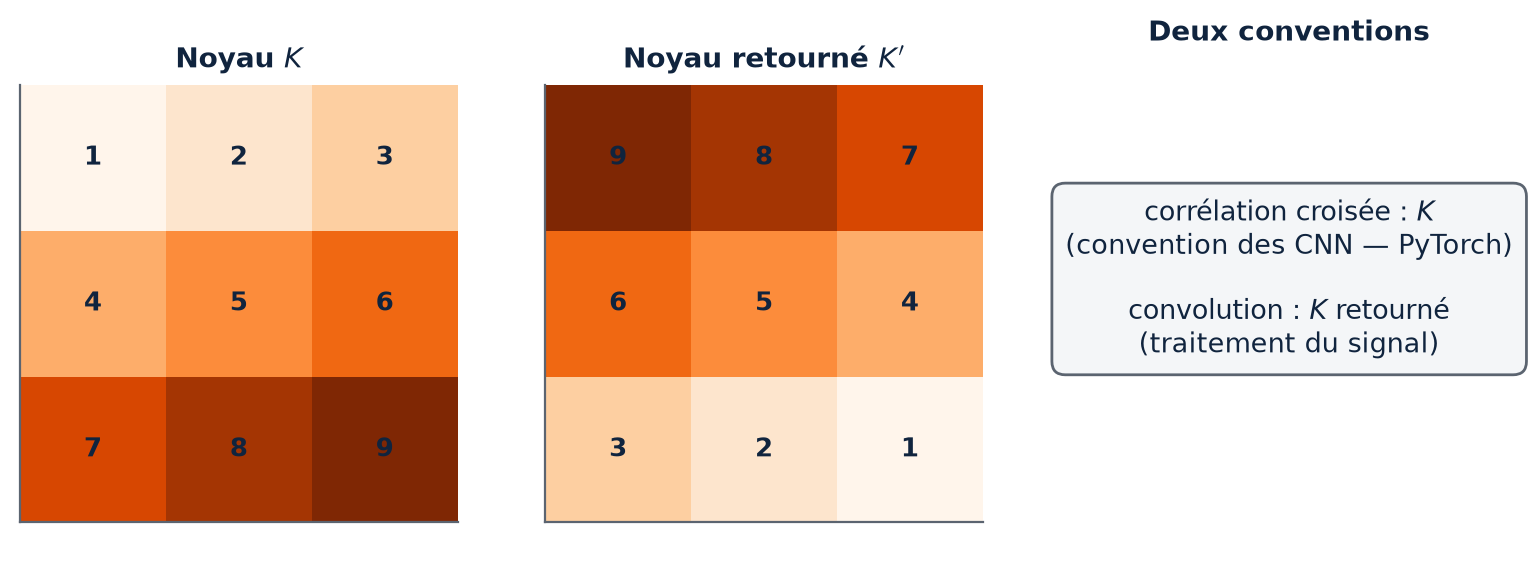
\includegraphics[width=0.46\textwidth]{g11_conv_vs_corr.png}
\end{center}
\end{column}
\begin{column}{0.43\textwidth}
\begin{kbox}[Deux conventions]
\textbf{Corrélation croisée} : on superpose le noyau $K$ tel quel.

\textbf{Convolution} (traitement du signal) : on retourne $K$ en $K'$ avant de
superposer.
\end{kbox}
\begin{wbox}[Le retournement]
Pour un noyau $3 \times 3$, retourner signifie lire la matrice à l'envers, à la fois
en ligne et en colonne : le $9$ passe en haut à gauche, le $1$ en bas à droite.
\end{wbox}
\end{column}
\end{columns}
\end{frame}

\begin{frame}{La convention de PyTorch, en pratique}
\begin{columns}[t]
\begin{column}{0.50\textwidth}
\begin{itemize}
  \item PyTorch (\file{nn.Conv2d}) implémente une \textbf{corrélation croisée}, pas un
  retournement de noyau.
  \item Pour un noyau \emph{symétrique}, les deux donnent le même résultat : le
  retournement est invisible.
  \item Pour un noyau non symétrique, la sortie de \file{convolve2d} est la version
  « miroir » de celle de PyTorch.
\end{itemize}
\end{column}
\begin{column}{0.46\textwidth}
\begin{kbox}[Pourquoi cela n'a aucune importance en apprentissage]
Le noyau est \textbf{appris}. Si la bonne réponse exige le noyau retourné, la descente
de gradient l'apprendra toute seule : retourner un noyau appris revient à apprendre le
noyau retourné. La convention n'est donc qu'une commodité de calcul.
\end{kbox}
\begin{abox}[Règle pratique pour ce cours]
On écrit la convolution comme la \emph{superposition directe} du noyau, c'est-à-dire
la convention de PyTorch, et on réserve le retournement à la théorie du signal.
\end{abox}
\end{column}
\end{columns}
\end{frame}

\begin{frame}{Intuition : ce que « voit » un noyau}
\begin{columns}[t]
\begin{column}{0.48\textwidth}
\begin{ebox}[Un noyau, une question posée à l'image]
\begin{itemize}
  \item Colonne de $+1$ et colonne de $-1$ : « y a-t-il un écart gauche/droite ? »
  \item Tous les coefficients égaux : « quelle est la moyenne locale ? »
  \item Centre fort et voisins négatifs : « cet endroit ressort-il ? »
\end{itemize}
\end{ebox}
\end{column}
\begin{column}{0.48\textwidth}
\begin{kbox}[Ce que la sortie conserve]
La sortie reste une \textbf{carte} : chaque valeur indique \emph{où} le motif a été vu.
C'est ce que le MLP perdait en aplatissant l'image, et ce que la convolution préserve.
Les noyaux classiques et leurs effets sont détaillés plus loin dans le chapitre.
\end{kbox}
\end{column}
\end{columns}
\end{frame}

\begin{frame}{À retenir et transition}
\begin{columns}[t]
\begin{column}{0.50\textwidth}
\begin{kbox}[À retenir]
\begin{itemize}
  \item Une convolution est un \textbf{calcul local} : produits terme à terme sur un
  voisinage, puis somme.
  \item Sur une image $5 \times 5$ et un noyau $3 \times 3$, la sortie est $3 \times 3$.
  \item Le \textbf{premier élément} de l'exemple vaut $0$, vérifié à la main et en code.
  \item Le même noyau \emph{glisse} partout : c'est le \emph{partage de poids}.
  \item \emph{Noyau}, \emph{filtre} et \emph{kernel} sont synonymes.
\end{itemize}
\end{kbox}
\end{column}
\begin{column}{0.48\textwidth}
\begin{wbox}[La question laissée ouverte]
Deux problèmes apparaissent dès qu'on généralise :
\begin{itemize}
  \item la sortie \emph{rétrécit} à chaque convolution ;
  \item on aimerait parfois \emph{sauter} des positions pour aller plus vite.
\end{itemize}
Ce sont le \textbf{padding} et le \textbf{stride}, objet de la partie suivante.
\end{wbox}
\end{column}
\end{columns}
\end{frame}